\capitulo{4}{Técnicas y herramientas}

Para el desarrollo del proyecto y para lograr alcanzar tanto los objetivos académicos como personales propuestos anteriormente, he considerado de utilidad las siguientes técnicas y herramientas.

\section{Gestión del proyecto y control de versiones}

\subsection{Gestión del proyecto}

A la hora de gestionar un proyecto, podemos clasificar el método usado para su gestión en dos grandes grupos: metodología tradicional y metodología ágil.

Analizando las diferencias entre ellas podemos afirmar~\cite{web:diferencias-metodologias}:

\begin{itemize}
	\item En la metodología tradicional, esta presente la figura de un Project Manager que basa sus conocimientos en el \textit{Project Management Body of Knowledge}\footnote{PMBoK. Libro donde se recogen técnicas y acciones a llevar a cabo dentro de un proyecto para obtener un resultado próspero.}.
	\item La metodología tradicional se centra en un enfoque proactivo y predictivo. Busca desde los orígenes del proyecto definir todo lo definible antes de empezar, anticiparse a cualquier cambio, buscar proyección, es decir, dar un alcance lo más completo posible y ajustar el coste al máximo.
	
	\item La metodología ágil surge como necesidad del cliente a proyectos no muy grandes. No existe una necesidad por parte del cliente de una planificación inicial exhaustiva, sino que necesita un producto en un espacio corto de tiempo y no hay tiempo para grandes planificaciones.
	\item Es probable que el producto demandado por el cliente en un principio, sea diferente del demandado a final del proyecto. Esto se debe al continuo cambio sobretodo en el mundo de las TIC. El cliente sabe qué necesita pero desconoce cómo se va a concretar a $X$ días vista
\end{itemize}

Estando delante de un proyecto no muy grande y aprovechando los conocimientos recibidos en el grado, hemos decidido utilizar una metodología ágil para gestionar nuestro proyecto.

\subsubsection{SCRUM}

\textit{Scrum}\footnote{No son siglas. Su significado viene de la palabra melé. Jugada de rugby en la que jugadores de ambos equipos se agrupan en una formación en la cual lucharán por obtener el balón que se introduce por el centro. \cite{web:scrum_origen}}~\cite{web:scrum} es uno de los métodos ágiles más extendidos. Se trata de un método incremental e iterativo que divide el desarrollo del producto en ciclos llamados \textit{sprints}.

Al inicio de cada \textit{sprint}, se realiza una reunión entre todos los integrantes del proyecto donde se definen los objetivos y requisitos de cada ciclo. Cada una de esas tareas se denomina \textit{issues}.

Este tipo de metodología ha sido muy eficiente en el desarrollo. Una de las ventajas que nos ha proporcionado, ha sido la capacidad de reaccionar ante los cambios teniendo la oportunidad de ir creando en cada \textit{sprint}, especificaciones y requerimientos nuevos.

\subsubsection{ZenHub}

\textit{ZenHub} es una plataforma de gestión de proyectos que se integra en \textit{GitHub}, instalándose en el navegador mediante una extensión \footnote{Podemos descargarlo en \url{https://www.zenhub.com/}}.

Es una herramienta muy cómoda y visual, ya que permite administrar todos los elementos comentados anteriormente característicos de la metodología SCRUM. Destacar que ZenHub llama a los \textit{sprints}, \textit{milestones}. El resto de nomenclatura es igual.

En la figura \ref{fig:ZenHub} tenemos presentes las diferentes columnas del \textit{tablero}. Este elemento, es de gran utilidad para clasificar por \textit{milestones}, cada \textit{issue}.

\begin{figure}[ht]
	\centering
	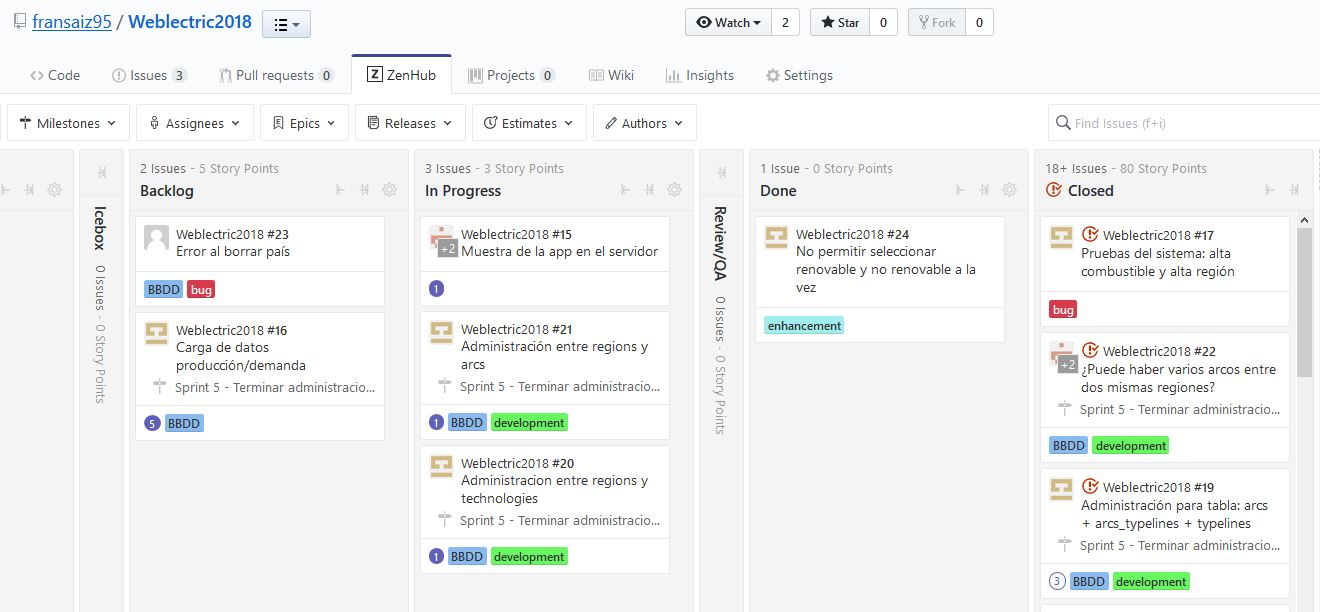
\includegraphics[width=1\textwidth]{/conceptosTeoricos/ZenHub}
	\caption{Ejemplo de nuestro tablero en \textit{ZenHub}.}
	\label{fig:ZenHub}
\end{figure}

\subsection{Control de versiones}

Como repositorio y control de versiones, hemos elegido \textit{Git} a través de la herramienta \textit{GitHub}\footnote{Software de código abierto y gratuito que permite un control de versiones a través de ramas (\textit{branchs}) en las que cada usuario puede editar y publicar cambios.}

GitHub es una plataforma online basada en Git, que permite la creación de repositorios tanto públicos como privados en los que posteriormente un equipo puede alojar su trabajo.

Además, GitHub ofrece una version para escritorio (\textit{GitHub Desktop}) con la que poder realizar subidas y bajadas (\textit{push - pull}) directamente desde el escritorio. Nosotros hemos utilizado \textit{Sourcetree}, un cliente Git que proporciona una interfaz amigable para interactuar con nuestros repositorios. Pertenece a la empresa \textit{Atlassian.}

A través del siguiente enlace, podemos acceder al proyecto \textit{Weblectric} que utiliza \textit{GitHub} como repositorio y control de versiones.

\url{https://github.com/fransaiz95/Weblectric2018}

\newpage

\section{Entorno de desarrollo}

Puesto que el objetivo principal del proyecto es construir una aplicación web dando soporte al cliente a que pueda cubrir sus necesidades, necesitamos un sitio donde alojar la aplicación. 

Antes de contratar ningún servicio externo, empezamos a desarrollar la aplicación en nuestro entorno local. Para ello necesitamos de la siguiente herramienta.

\subsection{XAMPP}

XAMPP es un paquete de software libre que consiste principalmente en el sistema de gestión de bases de datos \textit{MySQL}, el servidor web \textit{Apache} e intérpretes para lenguajes PHP y Perl~\cite{wiki:xampp}.

La ventaja de utilizar esta herramienta es que te ahorras el tiempo y la dificultad de configuración de cada uno de los servicios por separado. 

\subsection{HeidiSQL}

Aunque XAMPP trae consigo el servicio \textit{PhpMyAdmin} para gestionar las bases de datos \textit{MySQL}, nosotros hemos decidido utilizar \textit{HeidiSQL} ya que tiene una interfaz más amigable y permite más opciones.

\textit{HeidiSQL} es un software libre de código abierto que nos da la facilidad de conectarnos a servidores \textit{MySQL}.

Para administrar las bases de datos con esta herramienta, el usuario tiene que iniciar sesión en un servidor \textit{MySQL} local o remoto. 

\subsection{Filezilla}

Una vez que tenemos nuestro entorno de desarrollo en local, es común necesitar un servidor externo donde alojar tu aplicación. Para transferir los archivos al servidor, utilizamos \textit{Filezilla}. Un gestor \textit{FTP} de código abierto y software libre.

Tras establecer la conexión con el servidor, el manejo de los archivos y la navegación ente los directorios es fácil e intuitiva. Además, permite arrastrar y soltar, lo que facilita su uso.

\subsection{Visual Studio Code}

\textit{Visual Studio Code} es un editor de código fuente desarrollado por \textit{Microsoft}. Al incluir control integrado de \textit{Git}, hace que el resultado y el control de versiones de nuestro código sea más manejable.

No es un IDE como tal, pero gracias a numerosas extensiones hace que el trato con él sea mucho más satisfactorio. Acepta extensiones para hacer más fácil la lectura de los lenguajes \textit{PHP}, \textit{HTML}, \textit{CSS} y \textit{Javascript}. 



\subsection{Prepros}

\textit{Prepros} es una herramienta completa para desarrollo front-end\footnote{La parte del software que interactúa con los usuarios.}. Se trata de un compendio de funcionalidades que abarcan desde el desarrollo con lenguajes como CSS o Javascript, a la optimización de imágenes.

Además, en este trabajo, se utiliza como compilador de archivos \textit{*.scss} a \textit{*.css} pues el desarrollo se hace en \textit{Sass}, que es parecido a \textit{CSS}. Posteriormente se compila la estructura de archivos \textit{*.scss} en un \textit{*.css} general que utiliza la web.

Para una correcta estructuración de la hoja de estilos, en la figura \ref{fig:scss} podemos ver como se ha llevado a cabo.
Tenemos un directorio con cada uno de los archivos \textit{.scss} que se agrupan en un \textit{estilos.scss} que a su vez, siendo compilado con el \textit{Prepros}, genera un \textit{estilos.css}. Este archivo es de donde se nutre la aplicación web.

\begin{figure}[ht]
	\centering
	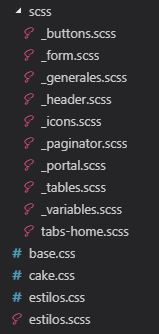
\includegraphics[width=0.3\textwidth]{/conceptosTeoricos/scss}
	\caption{Estructura de directorios de la hoja de estilos.}
	\label{fig:scss}
\end{figure}

\newpage

\section{Frameworks }

A continuación, iremos mencionando los diferentes \textit{frameworks (Entornos de trabajo)} que tras integrarlos entre sí, han hecho posible el desarrollo del proyecto.

\subsection{CakePHP}

\textit{CakePHP}~\cite{web:cakephp} es un \textit{framework} que facilita el desarrollo de aplicaciones web en PHP~\cite{wiki:cakephp}, utilizando el patrón de diseño MVC.

Facilita alguna ayuda para integrar \textit{Ajax}\footnote{Asynchronous JavaScript And XML (JavaScript asíncrono y XML), es una técnica de desarrollo web para crear aplicaciones interactivas~\cite{wiki:ajax}.}, Javascript, formularios... por lo que hace de su uso una herramienta interesante.

Además, vienen incluidos componentes de seguridad y de sesión que para una aplicación web siempre son interesantes.

En cuanto al Modelo Vista Controlador (figura~\ref{fig:mvc}), es un patrón de arquitectura de software que separa por una parte los datos y la lógica de una aplicación y por otra, la interfaz de usuario y el módulo encargado de gestionar los eventos y las comunicaciones. 

Separar las funciones de la aplicación en modelos, vistas y controladores hace que la aplicación sea mucho más ligera.

\begin{figure}[ht]
	\centering
	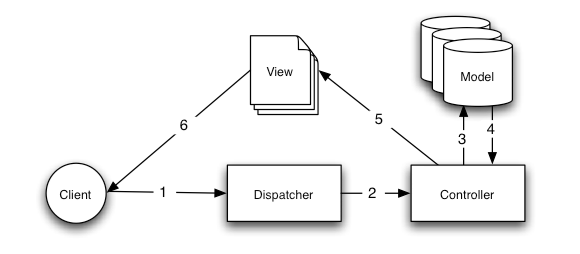
\includegraphics[width=0.9\textwidth]{/conceptosTeoricos/mvc}
	\caption{Ejemplo de arquitectura MVC. Ilustración extraida de~\cite{img:MVC}}
	\label{fig:mvc}
\end{figure}

\subsection{Zurb Foundation}

\textit{Foundation}~\cite{web:foundation} es un \textit{framework} de interfaz de usuario. Proporciona una cuadrícula responsive e incluye diferentes componentes:
\begin{itemize}
	\item Interfaz de usuario HTML y CSS.
	\item Plantillas.
	\item Fragmentos de código reutilizables.
	\item Tipografías.
	\item Formularios.
	\item Botones, barras de navegación y otros componentes de interfaz usuario.
	\item Extensiones de Javascript opcionales.
\end{itemize}

\textit{Foundation} está mantenida por \href{zurb.com}{Zurb} y es un proyecto de código abierto.

La competencia más directa de \textit{Foundation} como \textit{framework de CSS}, es \textit{Bootstrap}. Aunque en nuestra aplicación hemos usado \textit{Foundation}, cabe destacar que \textit{Bootstrap} ofrece unos servicios muy parecidos y una documentación de calidad como la de \textit{Foundation}. 

Por destacar alguna ventaja a favor de \textit{Bootstrap}, podemos decir que es más popular. Tiene más \textit{plugins} desarrollados y una comunidad de usuarios más grande, lo que facilita cualquier tipo de consulta en la web. Sin embargo, se ha decidido utilizar \textit{Foundation}, ya que viene con un archivo de ejemplo con el que hemos podido practicar y obtener conocimientos iniciales.
